\theoremstyle{definition}
\newtheorem{defn}{Definition}
\theoremstyle{plain}
\newtheorem{thm}{Theorem}
\theoremstyle{plain}
\newtheorem{lem}[thm]{Lemma}

\section{Formalisation in Type Theory}
\par Let us recall the two components of our formalisation: 1) the
translation of regular expressions to DFA and 2)
the correctness proofs of the translation. The translation in 1) is
divided into several steps. Firstly, any regular expression is
converted into an \(\epsilon\)-NFA using Thompson's construction
\cite{thompson1968}. Secondly, all the
\(\epsilon\)-transitions are removed by computing the
\(\epsilon\)-closures in order to get a NFA. Thirdly,
a DFA is built by using powerset construction. After that, all the unreachable
states are removed. Finally, a minimal DFA is obtained by using
quotient construction. In part 2), we prove
that accepting languages of the translated output are equal. i.e. \(L(regex) =
L(translated\ \epsilon\)-NFA\() = L(translated\) DFA\() =
L(translated\) MDFA\()\). Furthermore, we also need to prove that the translated
MDFA is minimal. 

\par In this section, we will walk through the formalisation of
each of the above steps together with their correctness proofs. Note
that all the definitions, theorems, lemmas and proofs written in this section
are adapted to the environment of Agda. Now let us begin with the 
representation of subsets and languages. 


\subsection{Subsets and Decidable Subsets}
\par Subset and decidable subset are defined in
\textbf{Subset.agda} and \textbf{Subset/DecidableSubset.agda}
respectively along with their operations such as membership (\(\in\)), subset
(\(\subseteq\)), superset (\(\supseteq\)) and equality (\(=\)). Let us
begin with the definition of general subsets. 

\begin{defn} 
\noindent Suppose \(A\) is a set, then its
subsets are represented as unary functions on
\(A\) in Type Theory, i.e. \(Subset\ A = A \to Set\). 
\end{defn}

\par In our definition, a subset is a function from \(A\) to
\(Set\). When declaring a subset, we can write \(sub =
\lambda\ (x : A) \to\ ?\). The \(?\) here should be replaced by the
conditions for \(x\) to be included in \(sub\). This construction is
very similar to set comprehension. For example, the subset 
\(\{x\ | \ x \in A,\ P(x)\}\) corresponds to \(\lambda\ (x : A) \to P\
x\). Furthermore, \(sub\) is also a predicate on \(A\) as it has the
type \(A \to Set\). As we have mentioned before, its decidability will
remain unknown until it is proved or disproved. 

\begin{defn} 
\noindent Another representation of subset is \(DecSubset\ A = A \to
Bool\). Unlike \(Subset\), its decidability is ensured by its
definition. 
\end{defn}

\par The two representations have different roles in the project. For
example, \(Language\) is definfed using \(Subset\) as not every
language is decidable. For other parts in the project 
such as the subsets of states in an automaton, \(DecSubset\) is used
because the decidability is assumed. 

\subsubsection{Operations on Subsets}
\par ...

\subsubsection{Operations on Decidable Subsets}
\par ...


\subsection{Languages}
\par Language is defined in \textbf{Language.agda} along with its 
operations and lemmas such as union \(\cup\), concatenation
\(\bullet\) and closure \(\star\). 

\par Suppose \(\Sigma\) is a set of alphabets, then it
can be represented as a data type in Type Theory, i.e. \(\Sigma :
Set\). Note that the equality of the set \(\Sigma\) needs to be
decidable. In Agda, they are passed to every module as
parameters in the form \((\Sigma : Set)\ (dec : DecEq\ \Sigma)\). 

\begin{defn}
\noindent We first define \(\Sigma^*\) as the set of all
strings over \(\Sigma\). In our approach, it is expressed as a list, i.e. \(\Sigma^* = List\ \Sigma\). 
\end{defn}

\par For example, (\(A :: g :: d :: a :: []\)) is equivalent to the string 'Agda' and the empty list \([]\)
represents the empty string (\(\epsilon\)). In this way, the first
alphabet of the input string can be extracted by pattern matching in order to
run a transition from a particular state to another state in an automaton. 

\begin{defn}
\noindent A language is defined as a subset of 
\(\Sigma^*\), i.e. \(Language = Subset\ \Sigma^*\). 
Note that \(Subset\) instead of \(DecSubset\) is used because not
every language is decidable. 
\end{defn}

\subsubsection{Operations on Languages}

\begin{defn} 
\noindent Suppose \(L_1\) and \(L_2\) are languages, then the union of
the two languages, \(L_1\cup L_2\), is defined as the set \(\{w\
|\  w \in L_1\ \vee \ w \in L_2\}\). In Type Theory, it is defined as \(L_1 \cup L_2 = \lambda\ w
\to w \in L_1\ \uplus\ w \in L_2\).
\end{defn}

\begin{defn}
\noindent Suppose \(L_1\) and \(L_2\) are languages, then
the concatenation of the two languages, \(L_1\bullet L_2\), is defined
as \(\{w\  |\  \exists u\in L_1.\ \exists v\in L_2.\ w = uv\}\). In
Type Theory, it is defined as \(L_1\bullet L_2 = \lambda\ w \to \exists[\
u \in \Sigma^*\ ]\ \exists[\ v \in \Sigma^*\ ] (u \in L_1 \times v \in
L_2 \times w \equiv u\ \Plus\Plus\  v )\).
\end{defn}

\begin{defn}
\noindent Suppose \(L\) is a language, then we define \(L\) \^\ \(n\) as
the concatenation of \(L\) with itself over \(n\) times. In Type Theory,
it is defined as a recursive function where \(L\) \^\ \(zero = [\![\epsilon ]\!]\) and
\(L\) \^\ \((suc\ n) = L \bullet L\) \^\ \(n\). 
\end{defn}

\begin{defn}
\noindent Suppose \(L\) is a language, then the closure of
L, \(L\ast\) is defined as \(\bigcup_{n \in N} L^n\). In Type
Theory, it is defined as \(L\ \star = \lambda\ w \to \exists [\ n \in \mathbb{N}\
](w \in L\) \^\ \(n)\). 
\end{defn}


\subsection{Regular Expressions and Regular Languages}
\par Regular expression and regular language are defined in
\textbf{RegularExpression.agda}. The set of alphabet \(\Sigma\) is
passed to the file as a parameter. 

\begin{defn}
\noindent Regular expressions over \(\Sigma\) are defined inductively as follow: 
\begin{enumerate}[nolistsep]
  \item \(\O\) is a regular expression denoting the regular language \(\O\);
  \item \(\epsilon\) is a regular expression denoting the regular language \(\{\epsilon\}\);
  \item \(\forall a\in\Sigma.\ a\) is a regular expression denoting the regular language \(\{a\}\);
  \item if \(e_{1}\) and \(e_{2}\) are regular expressions denoting the regular
    languages \(L_1\) and \(L_2\) respectively, then
    \begin{enumerate}[nolistsep]
      \item \(e_{1}\ |\ e_{2}\) is a regular expressions denoting the
        regular language \(L_1 \cup L_2\);
      \item \(e_{1}\cdot e_{2}\) is a regular expression denoting the
        regular language \(L_1\bullet L_2\);
      \item \(e_{1}^{\ *}\) is a regular expression denoting the regular
        language \(L_1\ \star\).
     \end{enumerate}
\end{enumerate}
\end{defn}

\par The interpretation of regular expression is intuitive:

\begin{lstlisting}[mathescape=true,xleftmargin=.3\textwidth]
data RegExp : Set where
  $\O$    : RegExp
  $\epsilon$    : RegExp
  $\sigma$    : $\Sigma$ $\to$ RegExp
  _|_ : RegExp $\to$ RegExp $\to$ RegExp
  _$\cdot$_  : RegExp $\to$ RegExp $\to$ RegExp
  _$^*$  : RegExp $\to$ RegExp
\end{lstlisting} 

\par The accepting language of regular expressions is defined as
a function from \(RegExp\) to \(Language\). 

\begin{lstlisting}[mathescape=true,xleftmargin=.3\textwidth]
L$^R$ : RegExp $\to$ Language
L$^R$ $\O$   = $\o$
L$^R$ $\epsilon$   = $[\![\epsilon ]\!]$
L$^R$ ($\sigma$ a) = $[\![\ a\ ]\!]$
L$^R$ (e$_1$ | e$_2$) = L$^R$ e$_1$ $\cup$ L$^R$ e$_2$
L$^R$ (e$_1$ $\cdot$ e$_2$) = L$^R$ e$_1$ $\bullet$ L$^R$ e$_2$
L$^R$ (e$^*$) = (L$^R$ e) $\star$
\end{lstlisting} 


\subsection{\(\epsilon\)-Non-deterministic Finite Automata}
\par Recall that the set of strings is defined as \(List\
\Sigma^*\). However, this definition gives us no way to
extract an \(\epsilon\)-transition from the input string. Therefore,
we need to introduce another representation specific to this purpose. 

\begin{defn}
\noindent We define \(\Sigma^e\) as the union of
\(\Sigma\) and \(\{\epsilon\}\), i.e. \(\Sigma^e = \Sigma \cup \{\epsilon\}\).
\end{defn} 

\par The equivalent data type is as follow:
\begin{lstlisting}[mathescape=true,xleftmargin=.3\textwidth]
data $\Sigma^e$ : Set where
  $\alpha$ : $\Sigma \to \Sigma^e$
  E : $\Sigma^e$
\end{lstlisting}

\par Alphabets in \(\Sigma\) are included in \(\Sigma^e\) by using the
\(\alpha\) constructor while the \(\epsilon\) alphabet correpsonds to \(E\)
in the data type. 

\begin{defn}
\noindent Now we define \(\Sigma^{e*}\), the set of all strings over
\(\Sigma^e\) in a way similar to \(\Sigma^*\), i.e. \(\Sigma^{e*} =
List\ \Sigma^e\). 
\end{defn}

\par For example, the string 'Agda' can be
represented by (\(\alpha\ A ::\ \alpha\ g :: E ::\ \alpha\ d :: E ::\ \alpha\
a :: []\)) or (\(E ::\ \alpha\ A :: E :: E ::\ \alpha\ g ::\ \alpha\ d :: E ::\ \alpha\
a :: []\)). We call these two lists as the \(\epsilon\)-strings of the
string 'Agda'. The definitions, operations and lemmas regarding
\(\epsilon\)-strings can be found in \textbf{Language.agda}. 

\par Now, let us define \(\epsilon\)-NFA using \(\Sigma^{e*}\). \(\epsilon\)-NFA is
defined in \textbf{eNFA.agda} along with its operations and
properties. 

\begin{defn}
\noindent An \(\epsilon\)-NFA is a 5-tuple \(M = (Q
,\ \Sigma^e,\ \delta,\ q_0,\ F)\), where
\begin{enumerate}[nolistsep]
  \item \(Q\) is a finite set of states;
  \item \(\Sigma^e\) is the union of \(\Sigma\) and \(\{\epsilon\}\);
  \item \(\delta\) is a mapping from \(Q \times\ \Sigma^e\) to
    \(\mathcal P \left({Q}\right)\) that defines the behaviour of the automata;
  \item \(q_0\) in \(Q\) is the initial state;
  \item \(F \subseteq Q\) is the set of accepting states. 
\end{enumerate}
\end{defn}

\par \(\epsilon\)-NFA is formalised in Agda as a record. 

\begin{lstlisting}[mathescape=true,xleftmargin=.3\textwidth]
record $\epsilon \hyphen$NFA : Set$_1$ where
  field
    Q      : Set
    $\delta$       : Q $\to$ $\Sigma^e$ $\to$ DecSubset Q
    q$_0$      : Q
    F      : DecSubset Q
    $\forall$qEq    : $\forall$ q $\to$ q $\in^d$ $\delta$ q E
    Q?     : DecEq Q
    |Q|-1  : $\mathbb{N}$
    It     : Vec Q (suc |Q|-1)
    $\forall$q$\in$It    : (q : Q) $\to$ (q $\in^V$ It)
    unique : Unique It
\end{lstlisting}

\par The set of alphabets \(\Sigma : Set\) is passed into the module as a
parameter. Together with \(Q\), \(\delta\),
\(q_0\) and \(F\), these five fields correspond to the 5-tuple
\(\epsilon\)-NFA. The other extra fields are used when computing
\(\epsilon\)-closures. They are \(\forall qEq\) -- a proof of the
lemma that says any state in \(Q\) can reach itself by an
\(\epsilon\)-transition; \(Q?\) -- the decidable equality of \(Q\);
\(|Q|-1\) -- the number of states minus 1; \(It\) -- a vector of
length \(|Q|\) that contains every state in \(Q\); \(\forall q\in It\)
-- a proof of the lemma that says every state in \(Q\) is also in the vector
\(It\) and \(unique\) -- a proof of the lemma that says there is no repeating elements in
\(It\). We will look into these extra fields with more details in
later part. 

\par In order to define the accepting language of a given
\(\epsilon\)-NFA, we need to define several operations of
\(\epsilon\)-NFA first. 

\begin{defn}
\noindent A configuration is composed of a state and an alphabet from
\(\Sigma^e\), i.e. \(C = Q \times \Sigma^{e*}\). 
\end{defn}

\begin{defn}
\noindent A move in an \(\epsilon\)-NFA \(N\) is
represented by a binary function \(\vdash\) on two configurations. We say
that \((q, aw) \vdash (q' , w)\) for all \(w \in \Sigma^{e*}\) and \(a \in \Sigma^e\)
 if and only if \(q' \in \delta (q , a)\). 
\end{defn}

\par The binary function is defined in Agda as follow: 
\begin{lstlisting}[mathescape=true]
  _$\vdash$_ : (Q $\times$ $\Sigma^e$ $\times$ $\Sigma^{e*}$) $\to$ (Q $\times$ $\Sigma^{e*}$) $\to$ Set
  (q , a , w) $\vdash$ (q' , w') = w $\equiv$ w' $\times$ q' $\in^d$ $\delta$ q a
\end{lstlisting}

\begin{defn}
\noindent Suppose \(C\) and \(C'\) are configurations. We say that \(C \vdash^0 C'\) if and only
if \(C = C'\). Also, \(C_0 \vdash^k C_k\) for any \(k \geq 1\) if and only if there exists a chain of
configurations \(C_1, C_2, ..., C_{k-1}\) such that \(C_i \vdash C_{i+1}\) for all \(0 \leq i \leq k\). 
\end{defn}

\par It is defined as a recursive function in Agda as follow: 
\begin{lstlisting}[mathescape=true]
  _$\vdash^k$_-_ : (Q $\times$ $\Sigma^{e*}$) $\to$ $\mathbb{N}$ $\to$ (Q $\times$ $\Sigma^{e*}$) $\to$ Set
  (q , w$^e$) $\vdash^k$ zero  - (q' , w$^e$')
    = q $\equiv$ q' $\times$ w$^e$ $\equiv$ w$^e$'
  (q , w$^e$) $\vdash^k$ suc n - (q' , w$^e$') 
    = $\exists$[ p $\in$ Q ] $\exists$[ a$^e$ $\in$ $\Sigma^e$ ] $\exists$[ u$^e$ $\in$ $\Sigma^{e*}$ ]
      (w$^e$ $\equiv$ a$^e$ :: u$^e$ $\times$ (q , a$^e$ , u$^e$) $\vdash$ (p , u$^e$) $\times$ (p , u$^e$) $\vdash^k$ n - (q' , w$^e$'))
\end{lstlisting}

\begin{defn}
\noindent We say that \(C \vdash^* C'\) if and only
if there exists a number of chains \(n\) such that \(C \vdash^n C'\). 
\end{defn}

\par Its corresponding type is defined as follow: 
\begin{lstlisting}[mathescape=true]
  _$\vdash^*$_ : (Q $\times$ $\Sigma^{e*}$) $\to$ (Q $\times$ $\Sigma^{e*}$) $\to$ Set
  (q , w$^e$) $\vdash^*$ (q' , w$^e$') = $\exists$[ n $\in$ $\mathbb{N}$ ] (q , w$^e$) $\vdash^k$ n - (q' , w$^e$')
\end{lstlisting}

\begin{defn}
\noindent For any string \(w\), it is accepted by an \(\epsilon\)-NFA \(N\)
if and only if there exists an \(\epsilon\)-string \(w^e\) of \(w\)
that can take \(q_0\) to an accepting state \(q\). 
\end{defn}

\begin{defn}
\noindent The language accepted by an
\(\epsilon\)-NFA is given by the set \(\{\ w\ |\ \exists w^e\in
\Sigma^{e*}.\ w = to\Sigma^*(w^e) \wedge \exists q\in F.\ (q_0\ ,\
w^e) \vdash^* (q\ ,\ \epsilon)\ \}\). 
\end{defn}

\par The correpsonding formalisation in Agda is defined as follow: 
\begin{lstlisting}[mathescape=true]
  L$^{eN}$ : $\epsilon \hyphen$NFA $\to$ Language
  L$^{eN}$ nfa = $\lambda$ w $\to$ 
            $\exists$[ w$^e$ $\in$ $\Sigma^{e*}$ ] (w $\equiv$ $to\Sigma^*$ w$^e$ $\times$ ($\exists$[ q $\in$ Q ] (q $\in^d$ F $\times$ (q$_0$ , w$^e$) $\vdash^*$ (q , []))))
\end{lstlisting} 

\par Now we can formulate the translation of regular
expressions to \(\epsilon\)-NFA using Thompson's Construction and
prove that their acceping languages are equal. 


\subsection{Thompson's Construction}
\par The translation of regular expressions to \(\epsilon\)-NFA is
defined in \textbf{Translation/RegExp-eNFA.agda}. 

\begin{defn}
\noindent The translation of regular expressions
to \(\epsilon\)-NFA is defined inductively as follow:
\begin{enumerate}[nolistsep]
  \item for \(\O\), we have \(M = (\{init\},\ \Sigma^e,\ \delta,\
    init,\ \O)\) and graphically \begin{center}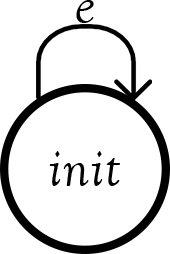
\includegraphics{null}\end{center}
  \item for \(\epsilon\), we have \(M = (\{init\},\ \Sigma^e,\
    \delta,\ init,\ \{init\})\) and graphically \begin{center}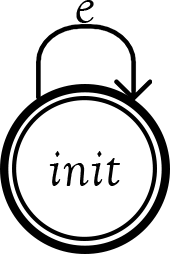
\includegraphics{epsilon}\end{center}
  \item for \(a\), we have \(M = (\{init, accept\},\ \Sigma^e,\
    \delta,\ init,\ \{accept\})\) and graphically \begin{center}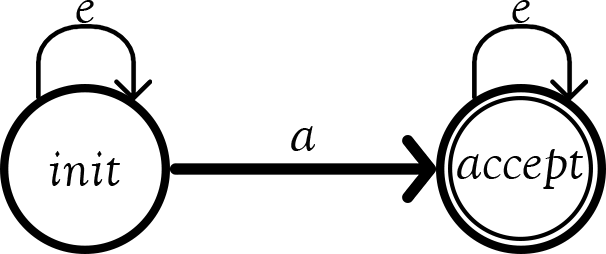
\includegraphics{singleton}\end{center}
  \item if \(N_1 = (Q_1,\ \delta_1,\ q_{01},\ F_1)\) and \(N_2 =
    (Q_2,\ \delta_2,\ q_{02},\ F_2)\) are \(\epsilon\)-NFAs translated from the
    regular expressions \(e_1\) and \(e_2\) respectively, then
    \begin{enumerate}[nolistsep]
      \item for \((e_1\ |\ e_2)\), we have \(M = (\{init\} \cup Q_1
        \cup Q_2,\ \Sigma^e,\ \delta,\ init,\ F_1 \cup F_2)\) and
        graphically \begin{center}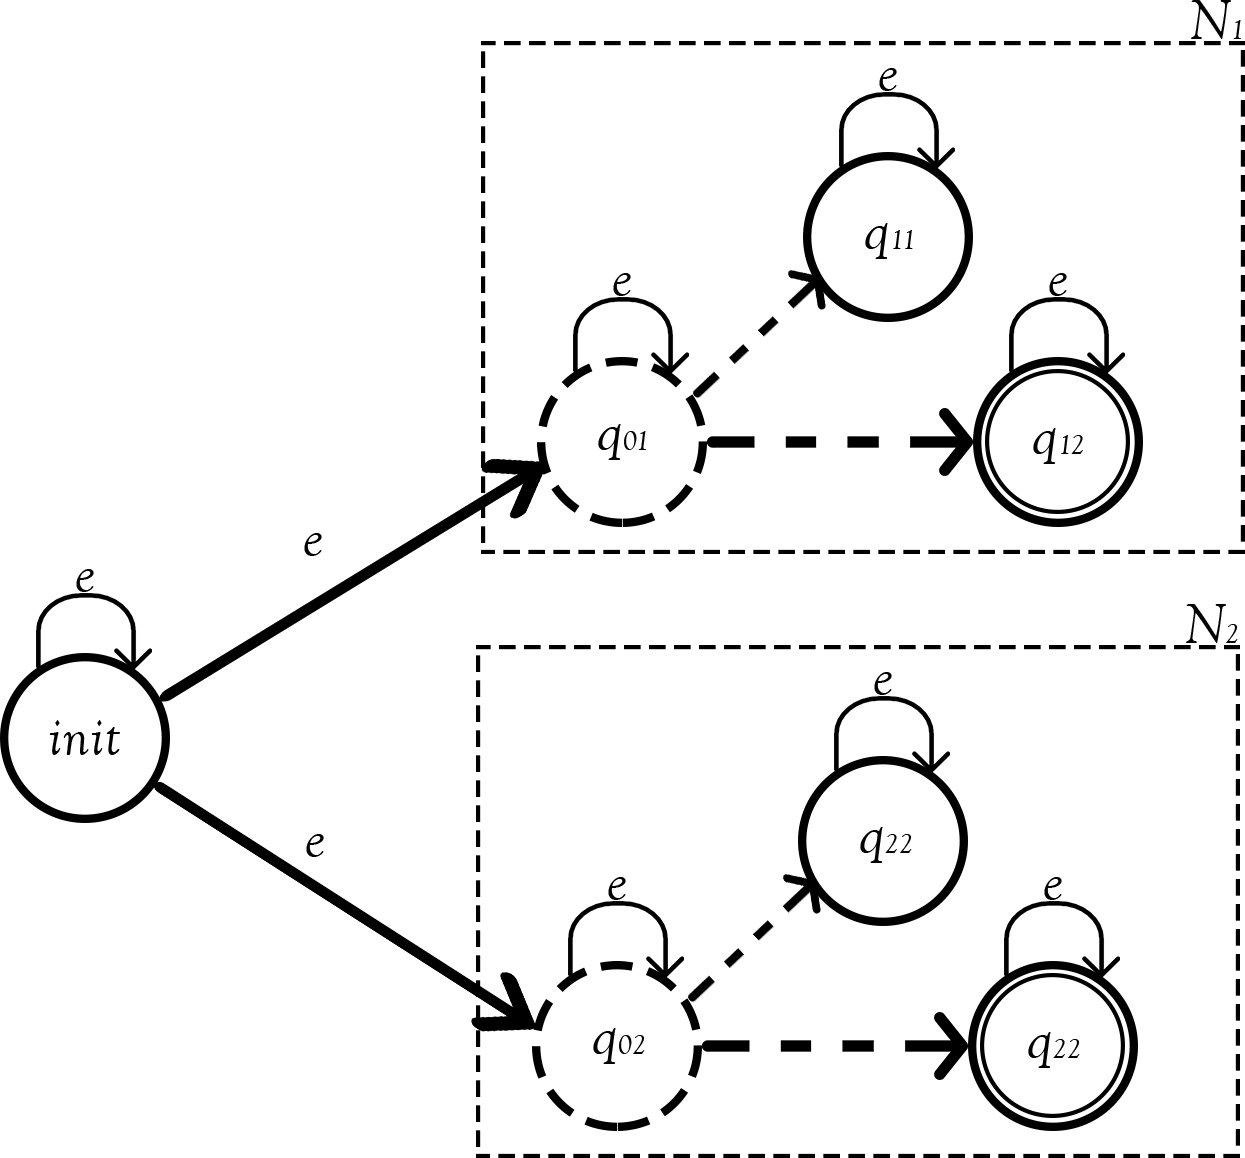
\includegraphics{union}\end{center}
      \item for \(e_1\cdot e_2\), we have \(M = (Q_1 \cup \{mid\}
        \cup Q_2,\ \Sigma^e,\ \delta,\ init,\ F_2)\) and graphically \begin{center}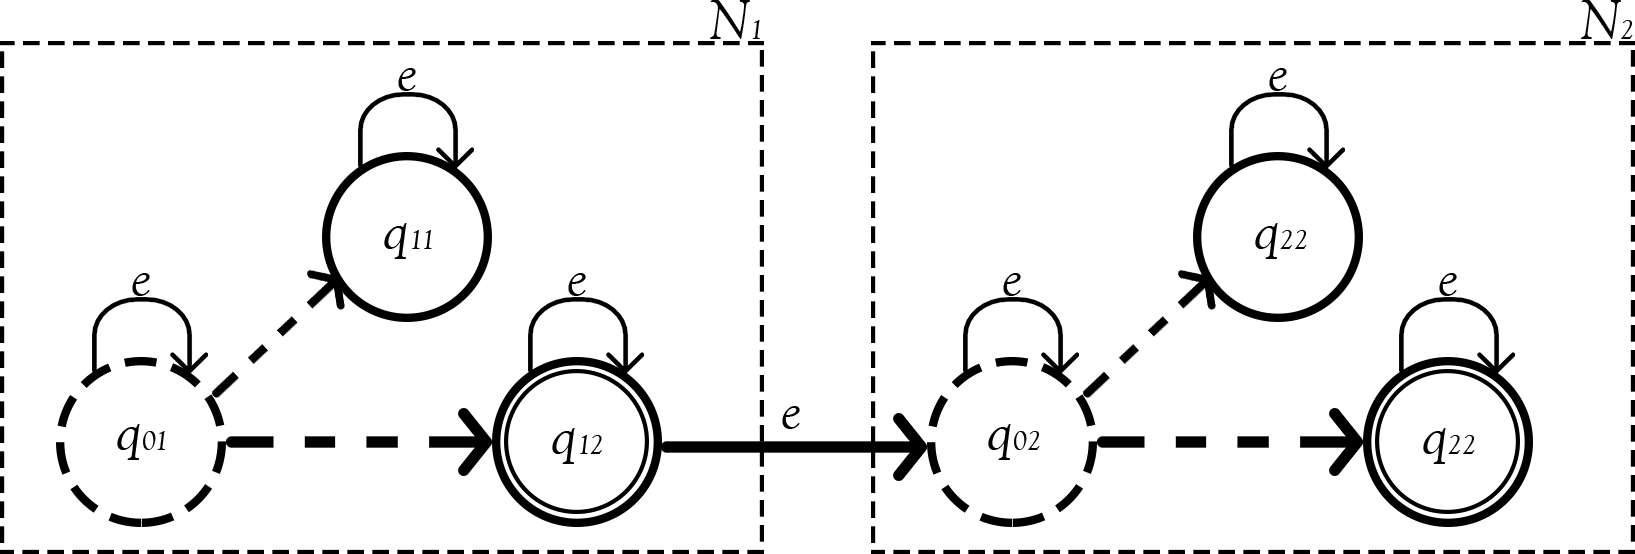
\includegraphics{concat}\end{center}
      \item for \(e_1^{\ *}\), we have \(M = (\{init\} \cup Q_1,\
        \Sigma^e,\ \delta,\ init,\ \{init\} \cup F_1)\) and
        graphically \begin{center}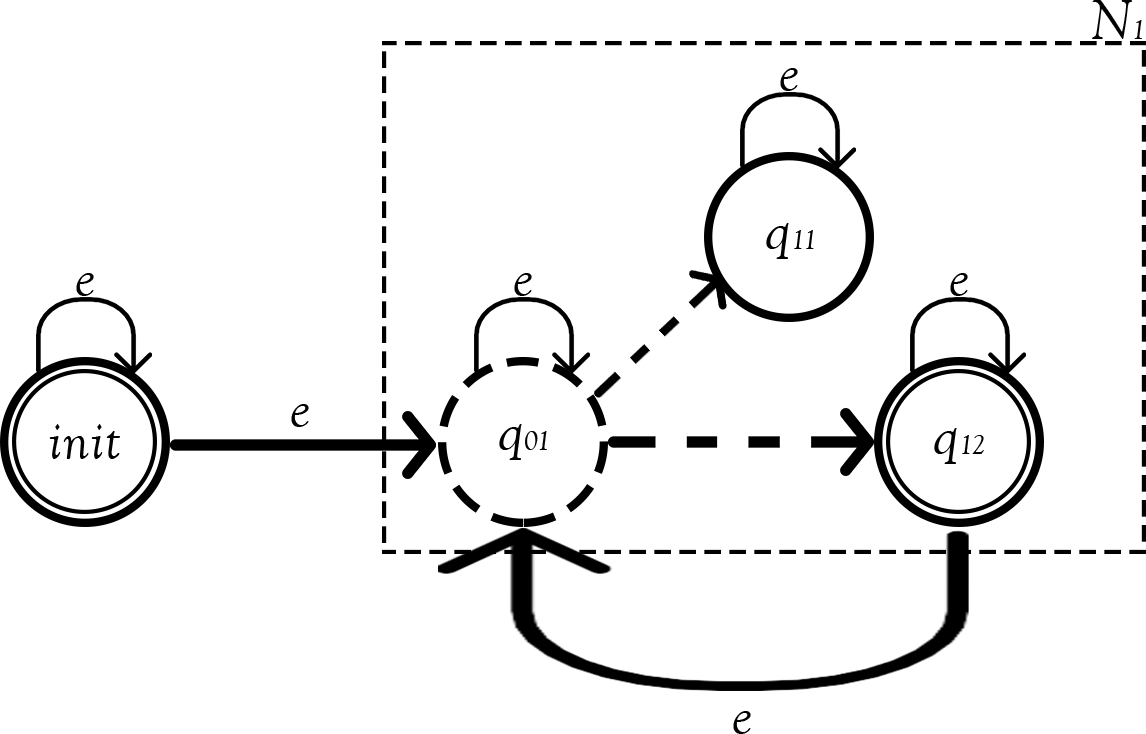
\includegraphics{star}\end{center}
     \end{enumerate}
\end{enumerate}
\end{defn}

\par Now, let us prove the correctness of the above translation by
proving their accepting languages are equal. The correctness proofs
are defined in \textbf{Correctness/RegExp-eNFA.agda}. 

\begin{thm} 
\noindent For any given regular expression \(e\), its accepting
language is equal to the language accepted by an \(\epsilon\)-NFA
translated from \(e\) using Thompson's Construction, i.e. \(L(e) =
L(translted\ \epsilon\)-NFA\()\). 
\end{thm} 

\begin{proof}
\noindent In order to prove the above theorem, we need to prove that
for any regular expression \(e\), \(L(e) \subseteq
L(translated\ \epsilon\)-\(NFA)\) and \(L(e) \supseteq L(translated\
\epsilon\)-\(NFA)\). They can be proved by induction on regular
expressions. 

\par \noindent \textbf{Base cases.}\quad By Definition ?, it is
obvious that the statement holds for \(\O\), \(\epsilon\) and
\(a\). 

\par \noindent \textbf{Induction hypothesis 1.}\quad For any two regular expressions
\(e_1\) and \(e_2\), let \(N_1 =
(Q_1,\ \delta_1,\ q_{01},\ F_1)\) and \(N_2 = (Q_2,\ \delta_2,\
q_{02},\ F_2)\) be their translated \(\epsilon\)-NFA 
respectively. We can assume that \(L(e_1) = L(N_1)\) and \(L(e_2) =
L(N_2)\). 

\par \noindent \textbf{Inductive steps.}\quad There are three cases 1)
\((e_1\ |\ e_2)\), 2) \((e_1 \cdot e_2)\) and 3) \((e_1\ ^*)\). 

\par \noindent 1) \textit{Case \((e_1\ |\ e_2)\)}: Let \(M = (Q,\ \delta,\ q_0,\ F) = (\{init\} \cup Q_1 \cup Q_2,\
\delta,\ init,\ F_1 \cup F_2)\) be its translated \(\epsilon\)-NFA. Then for any string \(w\), 

\par 1.1) if \((e_1\ |\ e_2)\) accepts \(w\), then by Definition ?,
either i) \(e_1\) accepts \(w\) or ii) \(e_2\) accepts \(w\). Assuming case i), then by
induction hypothesis, \(N_1\) also accepts \(w\) which implies that
there must exist an \(\epsilon\)-string \(w^e\) of \(w\) which can take \(q_{01}\)
to an accepting state \(q\) in \(N_1\). Now, we construct
another \(\epsilon\)-string of \(w\) by adding an \(\epsilon\) before the
\(\epsilon\)-string \(w^e\), i.e. \(\epsilon w^e\). The \(\epsilon\)-string \(\epsilon w^e\) can
take \(init\) to \(q\) in \(M\) because \(\epsilon\) can take \(init\)
to \(q_{01}\). Recall that \(q\) is an accepting
state in \(N_1\); therefore, \(q\) is also an accepting state in
\(M\). Now, we have proved that there exists an \(\epsilon\)-string
\(\epsilon w^e\) of \(w\) that can take \(init\) to an accepting state
\(q\) in \(M\); and thus \(M\) accepts \(w\). The same argument also applies
to other case when \(e_2\) accepts \(w\). Since we have proved that
\(w \in L(e_1\ |\ e_2)\) imples \(w \in L(M)\) for any string \(w\);
therefore \(L(e_1\ |\ e_2) \subseteq L(M)\) is true; 

\par 1.2) if \(M\) accepts \(w\), then there must exist an
\(\epsilon\)-string \(w^e\) of \(w\) which can take \(init\) to an
accepting state \(q\) in \(M\). \(q\) must be different from \(init\) because
\(q\) is an accepting state but \(init\) is not. Now, by Definition
?, there are only two possible ways for \(init\) to reach \(q\) in \(M\), i)
via \(q_{01}\) or ii) via \(q_{02}\). Assuming case i), then the head of \(w^e\)
must be an \(\epsilon\) because it is the only alphabet that can take
\(init\) to \(q_{01}\). Furthermore, \(q\) is an
accepting state in \(M\); therefore, \(q\) is also an accepting
state in \(N_1\). Now, let \(w^e = \epsilon u^e\), we have proved that
there exists an \(\epsilon\)-string \(u^e\) of \(w\) which can take
\(q_{01}\) to an accepting state \(q\) in \(N_1\); and thus \(N_1\)
accpets \(w\). By inductoin hypothesis, \(e_1\) also accepts \(w\);
therefore, we have \(w \in L(e_1\ |\ e_2)\). The same argument also
applies to case ii). Since we have proved that \(w \in L(M)\) implies
\(w \in L(e_1\ |\ e_2)\) for any string \(w\); therefore \(L(e_1\ |\
e_2) \supseteq L(M)\) is true; 

\par 1.3) combining 1.1 and 1.2, we have \(L(e_1\ |\ e_2) = L(M)\). 

\par \noindent 2) \textit{Case \((e_1 \cdot e_2)\)}: Let \(M = (Q,\
\delta,\ q_0,\ F) = (Q_1 \cup \{mid\} \cup Q_2,\ \delta,\ q_{01},\
F_2)\) be its translated \(\epsilon\)-NFA. Then for any string
\(w\), 

\par 2.1) if \((e_1 \cdot e_2)\) accepts \(w\), then by Definition
?, there must exist a string \(u \in L(e_1)\) and a string \(v \in L(e_2)\) such that \(w
= uv\). By induction hypothesis, \(N_1\) accepts \(u\) and \(N_2\)
accepts \(v\). Therefore, there must exist i) an \(\epsilon\)-string \(u^e\)
of \(u\) which can take \(q_{01}\) to an accepting state \(q_1\) in
\(N_1\) and ii) an \(\epsilon\)-string \(v^e\) of \(v\) which can take
\(q_{02}\) to an accepting state \(q_2\) in \(N_2\). Now, let us consider an \(\epsilon\)-string \(u^e\epsilon \epsilon
v^e\) of \(w\), \(u^e\epsilon \epsilon
v^e\) can take \(q_{01}\) to \(q_2\) in \(M\) because \(u^e\) takes
\(q_{01}\) to \(q_1\), \(\epsilon\) takes \(q_1\) to \(mid\), another
\(\epsilon\) takes \(mid\) to \(q_{02}\) and \(v^e\) takes \(q_{02}\)
to \(q_2\). Furthermore, \(q_2\)
is also an accepting state in \(M\) because \(q_2\) is an accepting
state in \(N_2\). Therefore, we have proved that \(M\) accepts \(w\). 
Since we have proved that \(w \in L(e_1 \cdot e_2)\) imples 
\(w \in L(M)\) for any string \(w\); therefore \(L(e_1 \cdot e_2) \subseteq L(M)\) is true; 

\par 2.2) if \(M\) accepts \(w\), then by Definition ?, there must
exist an \(\epsilon\)-string \(w^e\) of \(w\) which can take
\(q_{01}\) to an accepting state \(q\) in \(M\). Since \(q\) is an
accepting state in \(M\); therefore, \(q\) must be in \(Q_2\). The only possible way for
\(q_{01}\) to reach \(q\) is by going through the state \(mid\). This
implies that there must exist i) an \(\epsilon\)-string \(u^e\) which can take
\(q_{01}\) to an accepting state \(q_1\) in \(N_1\) and ii) an
\(\epsilon\)-string \(v^e\) which can take \(q_{02}\) to \(q_2\) in
\(N_1\). Let \(u\) and \(v\) be the normal strings of \(u^e\) and
\(v^e\) respectively, then we have \(u \in L(N_1)\), \(v \in L(N_2)\) and \(w = uv\). Now, by induction
hypothesis, \(e_1\) accepts \(u\) and \(e_2\) accepts \(v\); and thus
\(e_1 \cdot e_2\) accepts \(w\). Since we have proved that \(w \in
L(M)\) imples \(w \in L(e_1 \cdot e_2)\) for any string \(w\); therefore \(L(e_1 \cdot
e_2) \supseteq L(M)\) is true; 

\par 2.3) combining 2.1 and 2.2, we have \(L(e_1 \cdot e_2) = L(M)\). 

\par \noindent 3) \textit{Case \(e_1^*\)}: Let \(M = (Q,\ \delta,\ q_0,\
F) = (Q_1 \cup \{mid\} \cup Q_2,\ \delta,\ q_{01},\ F_2)\) be its
translated \(\epsilon\)-NFA. Then for any string \(w\), 

\par 3.1) if \((e_1\ ^*)\) accepts \(w\), then there must exist a number
\(n\) such that \(w \in (L\) \^\ \(n)\). Now, lets do induction on \(n\). 

\par \quad \textbf{Base case.} \quad When \(n = 0\), then language \(L\) \^\
\(0\) can only accept the empty string \(\epsilon\); and thus \(w =
\epsilon\). From Definition ?, it is obvious that \(M\) accepts
\(\epsilon\). 

\par \quad \textbf{Induction hypothesis 2.} \quad Suppose there exists a number \(k\) such that \(w
\in (L\) \^\ \(k\), then \(w\) is also accepted by \(M\). 

\par \quad \textbf{Induction steps.} \quad When \(n = k + 1\), by
Definition ?, there must exist a string \(u \in L(e_1)\) and a string \(v \in L(e_1)\)
\^\ \(k\) such that \(w=uv\). By induction hypothesis (1), we have \(u
\in L(N_1)\) which implies that there must exist an \(\epsilon\)-string
\(u^e\) of \(u\) that can take \(q_{01}\) to an accepting state \(q\)
in \(N_1\). Since \(q\) is an accepting state; an \(\epsilon\)
alphabet can take \(q\) back to \(q_{01}\). Furthermore, by induction
hypothesis (2), \(M\) also accepts \(v\) which implies that there exists an \(\epsilon\)-string \(v^e\) of \(v\)
that can take \(init\) to an accepting state \(p\). Since the only
alphabet that can take \(init\) to \(q_{01}\) is \(\epsilon\); therefore,
\(v^e\) must be in the form of \(\epsilon v^{e'}\). Now, we have proved
that there exists an \(\epsilon\) string \(\epsilon u^e\epsilon v^{e'}\) that can
take \(init\) to an accepting state \(p\) in \(M\); and thus \(M\)
accepts \(w\). Since we have proved that \(w \in L(e_1\ ^*)\) implies
\(w \in L(M)\) for any string \(w\); therefore \(w \in L(e_1\ ^*)
\subseteq L(M)\) is true; 

\par 3.2) if \(M\) accepts \(w\), then there must exist an
\(\epsilon\)-string \(w^e\) of \(w\) that can take \(init\) to an accepting
state \(q\) in \(M\).  If \(init = q\), then \(w\) must be an empty string. By Definition ?, it is obvious that
the empty string is accepted by \((e_1\ ^*)\). If \(init \neq q\),
then there are only two possible ways for \(init\)
to reach \(q\): 1) from \(init\) to \(q\) without any
transition that takes an accepting state in \(M\) back
to \(q_{01}\), we say that this path has no loops and 2) from \(init\)
to \(q\) with at least one transition that takes an accepting state in \(M\) back
to \(q_{01}\), we say that this path has loop. 
\par \quad \textit{Case 1}: Since \(q \neq init\), then \(w^e\) must
be in the form of \(\epsilon w^{e'}\). Recall that the path has no loops, it is
obvious that \(N_1\) accepts \(w\). Therefore by
induction hypothesis (1), \((e_1\ ^*)\) accepts \(w\) and thus \((e_1\
^*)\) also accepts \(w\). 
\par \quad \textit{Case 2}: Since \(q \neq init\), then \(w^e\) must
be in the form of \(\epsilon w^{e'}\). Recall that the path has loops, we
can separate the \(\epsilon\)-string into two parts: 1) a string
\(u^e\) that takes \(init\) to an accepting state \(p\) without loops
and 2) a string \(v^e\) that takes \(p\) to
\(q_{01}\) to \(q\) with loops. Let \(u\) and \(v\) be the normal
string of \(u^e\) and \(v^e\) respectively, then it is obvious that
\(w = uv\). By \textit{case 2}, \(e_1\) accepts \(u\). Also, by
induction, we can prove that there exists a number \(n\) such that
\((e_1)\) \^\ \(n)\) accepts \(v\). Combining the aboves, we have \(w \in
L(e_1\ ^*)\). 
\par Since we have proved that \(w \in L(M)\) implies \(w \in L(e_1\ ^*)\) for any string \(w\); therefore \(w \in
L(e_1\ ^*) \supseteq L(M)\) is true; 

\par 3.3) combining 3.1 and 3.2, we have \(L(e_1\ ^*) = L(M)\). 

\par Therefore, by induction, \(L(e) = L(translted\
\epsilon\)-NFA\()\) is true forall any regular expression \(e\). 
\end{proof}


\subsection{Non-deterministic Finite Automata}
\par Although the definition of NFA is very similar to that of
\(\epsilon\)-NFA, we will still define NFA separately for the sake of
integrity. NFA is defiend in \textbf{NFA.agda} along with its operations and properties. 

\begin{defn}
\noindent A NFA is a 5-tuple \(M = (Q
,\ \Sigma,\ \delta,\ q_0,\ F)\), where
\begin{enumerate}[nolistsep]
  \item \(Q\) is a finite set of states;
  \item \(\Sigma\) is the set of alphabets;
  \item \(\delta\) is a mapping from \(Q \times\ \Sigma\) to
    \(\mathcal P \left({Q}\right)\) which defines the behaviour of the automata;
  \item \(q_0\) in \(Q\) is the initial state;
  \item \(F \subseteq Q\) is the set of accepting states. 
\end{enumerate}
\end{defn}

\par It is formalised in Agda as a record. 

\begin{lstlisting}[mathescape=true,xleftmargin=.3\textwidth]
record NFA : Set$_1$ where
  field
    Q      : Set
    $\delta$       : Q $\to$ $\Sigma^e$ $\to$ DecSubset Q
    q$_0$      : Q
    F      : DecSubset Q
    Q?     : DecEq Q
    |Q|-1  : $\mathbb{N}$
    It     : Vec Q (suc |Q|-1)
    $\forall$q$\in$It    : (q : Q) $\to$ (q $\in^V$ It)
    unique : Unique It
\end{lstlisting}

\par The set of alphabets \(\Sigma : Set\) is passed into the module as a
parameter. Together with \(Q\), \(\delta\),
\(q_0\) and \(F\), these five fields correspond to the 5-tuple
\(\epsilon\)-NFA. \(Q?\) is
the decidable equality of \(Q\). \(|Q|-1\) is the number of states
minus 1. '\(It\)' is a vector of length \(|Q|\) containing all the
states in \(Q\). \(\forall q\in It\) is a
proof of the lemma -- all the states in \(Q\) are also in the vector
'\(It\)'. \(unique\) is a proof of the lemma -- there is no repeating elements in
'\(It\)'. These extra fields are important when performing powerset construction, we will look into them again in later part. 

\par Now, we want to define the set of strings \(\Sigma^*\) accepted by a given
NFA, but before that, we will first define several operations of NFA. 

\begin{defn}
\noindent A configuration is composed of a state and an alphabet from
\(\Sigma\), i.e. \(C = Q \times \Sigma\). 
\end{defn}

\begin{defn}
\noindent A move in an NFA \(N\) is
represented by a binary function \(\vdash\) on configurations. We say
that \((q, aw) \vdash (q' , w)\) for all \(w \in \Sigma\) and \(a \in \Sigma\)
 if and only if \(q' \in \delta (q , a)\). 
\end{defn}

%\par The corresponding type is defined as follow:
\begin{lstlisting}[mathescape=true]
  _$\vdash$_ : (Q $\times$ $\Sigma$ $\times$ $\Sigma$) $\to$ (Q $\times$ $\Sigma$) $\to$ Set
  (q , a , w) $\vdash$ (q' , w') = w $\equiv$ w' $\times$ q' $\in^d$ $\delta$ q a
\end{lstlisting}

\begin{defn}
\noindent Suppose \(C\) and \(C'\) are configurations. We say that \(C \vdash^0 C'\) if and only
if \(C = C'\). Also, \(C_0 \vdash^k C_k\) for any \(k \geq 1\) if and only if there exists a chain of
configurations \(C_1, C_2, ..., C_{k-1}\) such that \(C_i \vdash C_{i+1}\) for all \(0 \leq i \leq k\). 
\end{defn}

%\par In Agda, it is defined as a recursive function as follow:
\begin{lstlisting}[mathescape=true]
  _$\vdash^k$_-_ : (Q $\times$ $\Sigma$) $\to$ $\mathbb{N}$ $\to$ (Q $\times$ $\Sigma$) $\to$ Set
  (q , w) $\vdash^k$ zero  - (q' , w')
    = q $\equiv$ q' $\times$ w$^e$ $\equiv$ w$^e$'
  (q , w) $\vdash^k$ suc n - (q' , w') 
    = $\exists$[ p $\in$ Q ] $\exists$[ a $\in$ $\Sigma$ ] $\exists$[ u $\in$ $\Sigma$ ]
      (w $\equiv$ a :: u $\times$ (q , a , u) $\vdash$ (p , u) $\times$ (p , u) $\vdash^k$ n - (q' , w'))
\end{lstlisting}

\begin{defn}
\noindent We say that \(C \vdash^* C'\) if and only
if there exists a number of chains \(n\) such that \(C \vdash^n C'\). 
\end{defn}

%\par Its corresponding type is defined as: 
\begin{lstlisting}[mathescape=true]
  _$\vdash^*$_ : (Q $\times$ $\Sigma$) $\to$ (Q $\times$ $\Sigma$) $\to$ Set
  (q , w) $\vdash^*$ (q' , w') = $\exists$[ n $\in$ $\mathbb{N}$ ] (q , w) $\vdash^k$ n - (q' , w')
\end{lstlisting}

\begin{defn}
\noindent For any string \(w\), it is accepted by an NFA \(N\)
if and only if \(w\) can take \(q_0\) to an accepting state \(q\). 
\end{defn}

\begin{defn}
\noindent The language accepted by an NFA is given by the set \(\{\ w\
| \exists q\in F.\ (q_0\ ,\ w) \vdash^* (q\ ,\ \epsilon)\ \}\). 
\end{defn}

%\par ... 
\begin{lstlisting}[mathescape=true]
  L$^N$ : NFA $\to$ Language
  L$^N$ nfa = $\lambda$ w $\to$ $\exists$[ q $\in$ Q ] (q $\in^d$ F $\times$ (q$_0$ , w) $\vdash^*$ (q , []))))
\end{lstlisting} 

\par Now we can formulate the translation of \(\epsilon\)-NFA to NFA
by removing all the \(\epsilon\)-transitions. 


\subsection{Removing \(\epsilon\)-transitions}
\par The translation of \(\epsilon\)-NFA to NFA is defined in
\textbf{eNFA-NFA.agda}. In order to remove all the \(\epsilon\)-transitions, we need to
know whether a state \(q\) can reach another state \(q'\) with only
\(\epsilon\) transitions. 

\begin{defn}
\noindent We say that \(q \to_\epsilon^0 q'\) if and only if
\(q\) is equal to \(q'\). Also, \(q \to_\epsilon^k q'\) for \(k >
1\) if and only if there exists a state \(p\) such that \(p \in
\delta (q,\ \epsilon)\) and \(p \to_\epsilon^{k-1} q'\). 
\end{defn}

\begin{lstlisting}[mathescape=true]
_$\to_\epsilon^k$_-_ : Q $\to$ $\mathbb{N}$ $\to$ Q
q $\to_\epsilon^k$ zero - q' = q $\equiv$ q'
q $\to_\epsilon^k$ suc n - q' = $\exists$[ p $\in$ Q ] ( p $\in^d$ $\delta$ q E $\times$ p $\to_\epsilon^k$ n - q' )
\end{lstlisting}

\begin{defn}
\noindent We say that \(q \to_\epsilon^* q'\) if and only if there
exists a number \(n\) such that \(q \to_\epsilon^n q'\). 
\end{defn}

\begin{lstlisting}[mathescape=true]
_$\to_\epsilon^*$_ : Q $\to$ Q
q $\to_\epsilon^*$ q' = $\exists$[ n $\in$ $\mathbb{N}$ ] q $\to_\epsilon^k$ n - q'
\end{lstlisting}

\par Now we have to prove that for any pair of states (\(q,\ q'\)),
\(q \to_\epsilon^* q'\) is decidable. 



\subsection{Deterministic Finite Automata}
\par ...


\subsection{Powerset Construction}
\par ...


\subsection{Minimal DFA}
\par ...


\subsection{Minimising DFA}
\par ...

\subsubsection{Removing unreachable states}
\par ...

\subsection{Quotient construction}